\documentclass[conference]{IEEEtran}
%\IEEEoverridecommandlockouts
% The preceding line is only needed to identify funding in the first footnote. If that is unneeded, please comment it out.
\usepackage{cite}
\usepackage{amsmath,amssymb,amsfonts}
\usepackage{algorithmic}
\usepackage{graphicx}
\usepackage{textcomp}
\usepackage{url}
\renewcommand*\descriptionlabel[1]{\hspace\leftmargin$#1$}
\usepackage{xcolor}
\def\BibTeX{{\rm B\kern-.05em{\sc i\kern-.025em b}\kern-.08em
  T\kern-.1667em\lower.7ex\hbox{E}\kern-.125emX}}
   
   
\setcounter{secnumdepth}{5}
\setcounter{tocdepth}{5}

\makeatletter
\newcommand\subsubsubsection{\@startsection{paragraph}{4}{\z@}{-2.5ex\@plus -1ex \@minus -.25ex}{1.25ex \@plus .25ex}{\normalfont\normalsize\bfseries}}
\newcommand\subsubsubsubsection{\@startsection{subparagraph}{5}{\z@}{-2.5ex\@plus -1ex \@minus -.25ex}{1.25ex \@plus .25ex}{\normalfont\normalsize\bfseries}}
\makeatother

\newcommand{\ulsi}[1]{\!\overline{\,{#1}}} % underline short italic
\newcommand{\uls}[1]{\mskip.5\thinmuskip\underline{\mskip-.5\thinmuskip {#1} \mskip-.5\thinmuskip}\mskip.5\thinmuskip} % underline short
  
\begin{document}

\title{Linear Regression: Deep Learning}

\author{\IEEEauthorblockN{Olaniyi Bayonle Alao}
\IEEEauthorblockA{\textit{Summer Term, 2021} \\
\textit{Bachelor of Electronic Engineering} \\
\textit{Hochschule Hamm-Lippstadt}\\
Lippstadt, Germany \\
olaniyi-bayonle.alao@stud.hshl.de}
}

\maketitle

\begin{abstract}
Machine learning refers to applications' ability to get better at doing things without necessarily changing the codebase.
Even though machine learning is not a new concept, it is fast gaining recognition and changing lives thanks to the increase in the processing power of computers over the years to process big data at a level that has never been experienced. This paper talks about linear regression in the context of machine learning. Linear regression is a statistical term that uses a dependent and independent variable to make predictions. This paper explores the theoretical background of linear regression, solves a regression problem using machine learning for training a model, and predicts values using the trained model using Scikit-Learn, a scientific library for machine learning in python.
The paper uses the California housing datasets from the Scikit-Learn dataset repository for training the linear regression machine learning model. As a measure of how good the machine learning model has learnt, mean squared error and coefficient of determination were explained and determined. In conclusion, the paper evaluates the trained linear regression model to understand how well it performed in making predictions.
\end{abstract}
\begin{IEEEkeywords}
machine learning, linear regression, deep learning, sci-kit
\end{IEEEkeywords}


\section{Introduction}
Due to an explosive increase in the amount of data generated from different internet-connected devices - Cyber-Physical-Systems (CPS) -, there has been an increase in the need to make sense of this "big data" to ensure the proper and productive functioning of businesses. By 2026, the data generated from the global air fleet is projected to reach 98 billion gigabytes \cite{oliver_wyman}. Thanks to the recent advancements in the information processing capabilities of computers, making sense of this enormous chunk of data is now possible using data analysis techniques and machine learning algorithms to clean and make a prediction from these datasets. Machine learning is a machine's - software application - ability to learn and make predictions without being programmed to do so. They are able to learn and get better with an increase in the amount of data they are being fed through their grounded mathematical foundations.

\quad Linear regression is a statistical test used to ascertain the relationship between independent and dependent variables in a dataset using a mathematical formula. They can also be used in projecting a new relationship between the dependent and independent variables that have not been discovered.
Even though linear models - linear regression - are pretty simple to develop and understand, as well as good at predicting linear relationships, their approximation of nonlinear relationships is mostly unsatisfactory \cite{article_lee}. 

\quad This paper gives a profound yet understandable mathematical description of Linear regression. Relevant parts of the scientific machine learning framework -SciKit Learn- used to perform linear regression predictions on the example dataset in machine learning using Python programming language. 

\quad The theoretical background section of this paper gives in-depth information about fundamental theories in understanding the machine learning field and linear regression. The algorithm implementation section of the paper discusses the libraries and dataset used in implementing the linear regression machine learning model trained in this paper. A practical example of preparing the dataset, splitting the dataset, training the machine learning model, as well as testing out the trained model, its accuracy and interpretation of the predictions were presented in the practical and result and discussion section of the paper.

Unless otherwise stated, the main reference for facts, mathematical models and terminologies used in this research paper is from \cite{massaron2016regression}.
\section{Theoretical Background}
\subsection{Machine Learning}
According to \cite{ibm_cloud_education_2020}, "Machine learning is a branch of artificial intelligence (AI) focused on building applications that learn from data and improve their accuracy over time without being programmed to do so". Examples of applications built using machine learning trained models are email filters with the ability to distinguish between desired emails and spams, auto-suggestion/auto-correct in many typing applications, self-driving vehicles, amongst others. Machine learning techniques have the advantage of automatically adapting to change detected in trends from data. Likewise, they help reduce the complexity of writing applications that are sometimes difficult or even impossible to implement using conventional algorithms. The approach of solving an application's complexity using machine learning is shown in figure \ref{fig:machine_approach}. As depicted in figure \ref{fig:machine_approach}, machine learning algorithms do the job of find solutions to the studied problem and evaluation of the solution is done before being deployed. Methods used in training a Machine learning model can be grouped into three main categories.

\newpage
\begin{figure}[htbp]
	\centerline{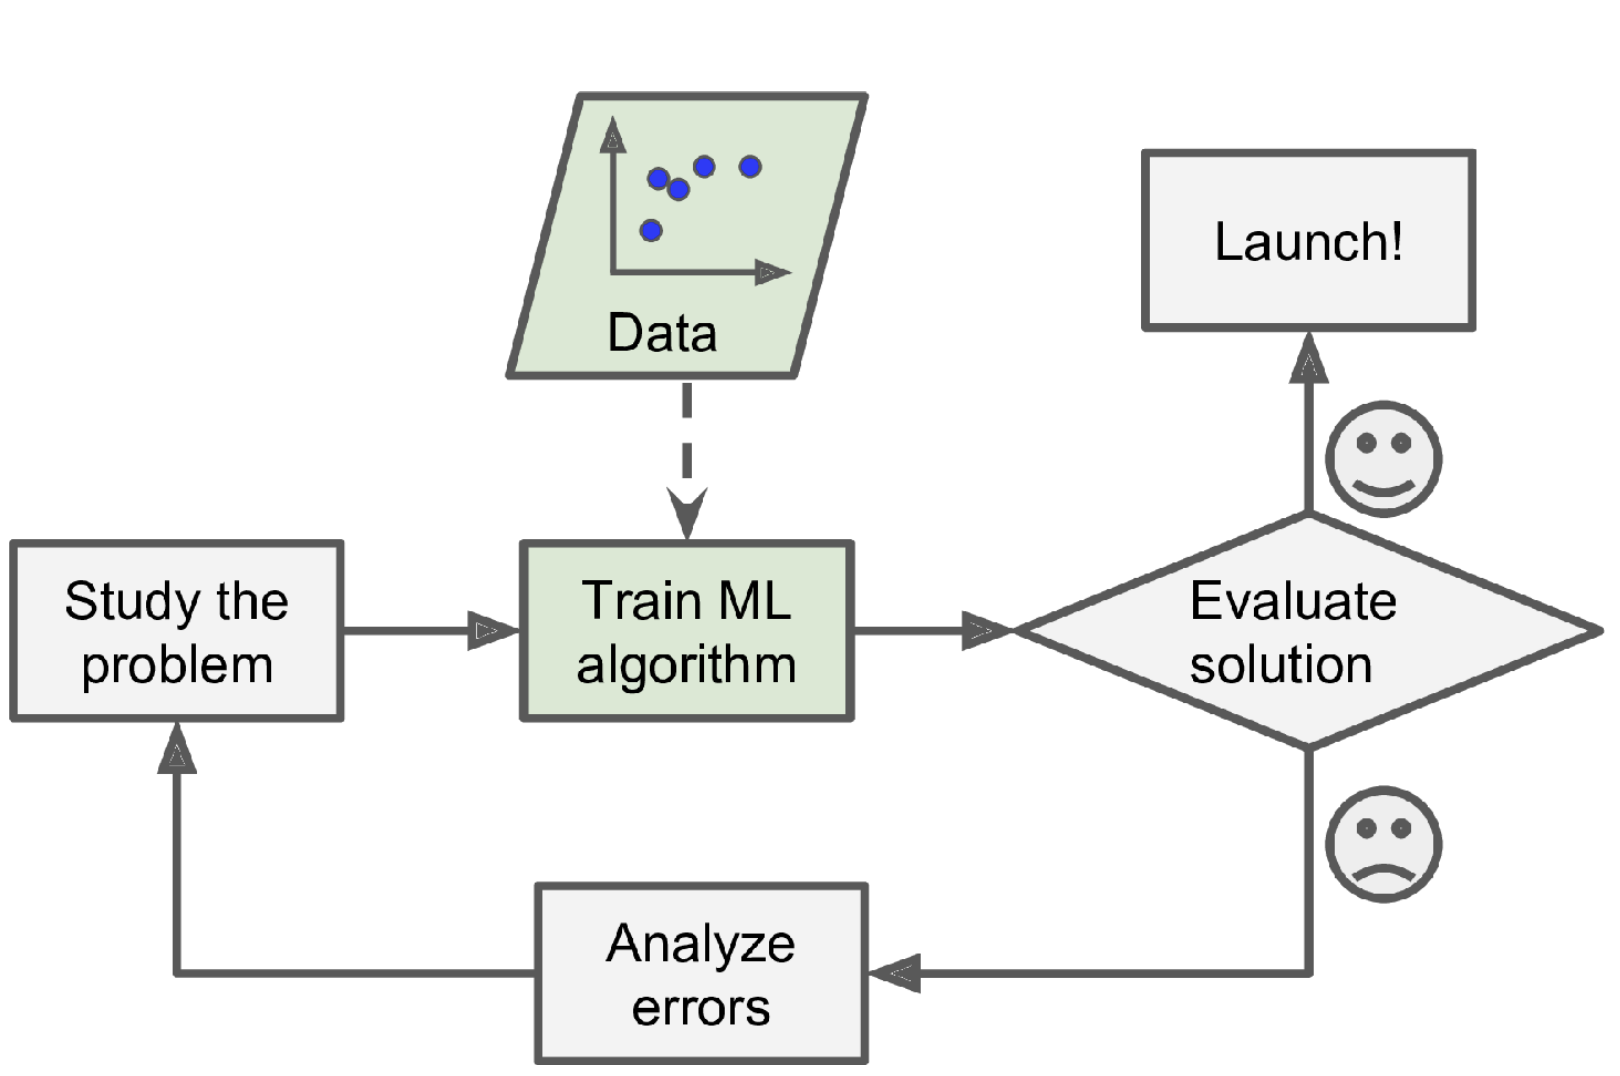
\includegraphics [scale=0.32]{figures/machine_approach.png}}
	\caption{Machine Learning approach \cite{geron2019hands}}
	\label{fig:machine_approach}
\end{figure}


	\begin{itemize}
		\item Supervised Learning
		
		This is a type of machine learning technique in which the algorithm is fed with an input and output dataset of the desired solution. The desired output data is otherwise known as labels. This information help train the machine learning model in the precise output prediction when given a related output after being trained. Some examples of standard algorithms used for supervised learnings are regression analysis - linear regression, logistic regression -, decision trees.\cite{theobald2017machine} The two kinds of supervised learning techniques used are classification and regression.
		\item Unsupervised Learning
		
		This refers to the machine learning technique in which the algorithm is only fed with input data for the training process. The model learns "unsupervised" by finding out and grouping patterns in inputted datasets. Unlike supervised learning, they require many unlabeled datasets to train - properly find patterns in datasets.
		\item Semisupervised Learning
		
		This learning technique uses both labeled - input and desired output - and unlabeled - only input - datasets for training machine learning models.
	\end{itemize}
The other methods used in training a machine learning model are reinforcement learning and deep learning. Deep learning is a subset of machine learning whose algorithm defines an artificial neural network - ANN - that is designed to emulate the way a human brain learns and uses unsupervised or semisupervised learning technique to train \cite{ibm_cloud_education_2020}. On the other hand, reinforcement learning is reward-based learning because the machine learning model is trained by being given a point for reaction to specific events.

\subsection{Linear Regression Model}
Regression 
is a predictive analysis with a long but glorious history from its successful applications to problems in the statistics and economics domain. Regression is a kind of supervised learning technique for determining the best fit line to describe patterns in data: linear regression uses a straight line to describe these patterns.\cite{theobald2017machine}. The best fit line is the line that reduces the summed squared difference between the value of the line of a certain value \textbf{\textit{x}} and its corresponding \textbf{\textit{y}} values \cite{massaron2016regression}. The mathematical expression for linear regression is:
	\begin{equation}
		y = \beta\label{beta}X + \beta\textsubscript{0}
	\end{equation}
	Where y is the dependent variable, X is the independent variable of the equation, $\beta$ is a cofficient which reperesnts the slope of the regression line, $\beta$\textsubscript{0} is a constant value called the \textbf{bias}. Equation \eqref{beta} is the same as the equation of a straight line in linear algebra.
	
	The independent variable X in \eqref{beta} is calculated using the mathematical expression below:
	\begin{equation}
  		%\frac{\sum{(x-x)(y-y)}{6}
		X = \frac{\sum{}(x-\overline{x})(y-\overline{y})}{\sum{}(x-\overline{x})^2}
		%\sum{}\frac{(x-x)}{5}
	\end{equation}	
	Where $\overline{x}$ and $\overline{y}$ are the mean values of all the respective x and y variables.
	
	
Linear regression analysis can be sub-divided into simple and multiple linear regression depending on the number of their independent variables. If the independent variable is one, the regression is a simple linear regression, but it is multiple linear regression if the independent variable is more than one. In this paper, we will make an analysis using the multiple linear regression model.

\subsection{Pearson's Correlation Coefficient}
According to \cite{ref1_pearson}, "Pearson's correlation coefficient (r) is a measure of the linear association of two variables". Equation \eqref{betas} shows the formula for calculating Pearson's correlation coefficient 
	\begin{equation}
  		%\frac{\sum{(x-x)(y-y)}{6}
		r = \frac{\sum{}(x-\overline{x})(y-\overline{y})}{\sqrt{\sum{}(x-\overline{x})^2\sum{}(y-\overline{y})^2}}\label{betas}
		%\sum{}\frac{(x-x)}{5}
	\end{equation}	
	Where:
	\begin{description}
		\item x = values of the x variable
		\item y = values of the y variable
		\item $\overline{x}$ = mean values of all the x variables
		\item $\overline{y}$ = mean values of all the y variables
		\item r = pearson's correlation coefficient
	\end{description}
	 
Correlation analysis usually starts with a graphical representation of the relation of data pairs using a scatter diagram. The correlation coefficient varies from a value of –1 to +1. A value of 1 indicates that the linear model accurately describes the relationship between the dependent and independent variables. The lower the value gets towards the negative value indicates that the dependent variable decreases with an increase in the value of the independent variable, meaning that there is a negative linear correlation between the variables.
The correlation coefficient value of 0 indicates no correlation between the dependent and independent variables.
\subsection{Model Evaluation}
The prediction made by the model using equation \eqref{beta} can be evaluated using the statistical methods below to find out how close the predicted value is to the actual value.
\subsubsection{R\textsuperscript{2}}
otherwise known as the coefficient of determination or the coefficient of multiple determination, which is a measure of how close the best fit line is to the original data using a simple mean. The value of the output of this calculation ranges from 0 to 1\cite{DAE79009}. A value of 1 refers to the fact that all the points fit 100$\%$ to the regression line. The lesser the value, the farther the points are to the regression line. The following equation defines the coefficient of determination:

	\begin{equation}
  		%\frac{\sum{(x-x)(y-y)}{6}
		R\textsuperscript{2} = \label{three}\frac{\sum_{i=1}^{n}(\hat{y_i}-\overline{y})^2}{\sum_{i=1}^{n}(y_i-\overline{y})^2}
		%\sum{}\frac{(x-x)}{5}
	\end{equation}
	
	Where n is the number of observations, i.e. total number of variables, $\hat{y_i}$ is the estimated value of the dependent variable for the i\textsuperscript{th} observation computed by the regression equation, $y_i$ is the observed value of the dependent variable for the i\textsuperscript{th} observation and $\overline{y}$ is the mean of all n observations of the dependent variable \cite{DAE79009}

\subsubsection{Mean Squared Error}
Mean Squared Error (MSE) is a performance measure that helps determine how much error is made in the predicted value in relation to the actual value of the output given the same input. The equation of the calculation is denoted by:

	\begin{equation}
  		%\frac{\sum{(x-x)(y-y)}{6}
		MSE = \label{four}\frac{1}{n}\sum_{i=1}^{n}(y_i-\hat{f}(x_i))^2
		%\sum{}\frac{(x-x)}{5}
	\end{equation}
	where $x_i$ is a vector of all i\textsuperscript{ith} observation, $\hat{f}$ is the prediction function. The lower the value of MSE, the more accurate the prediction is.
\section{Algorithm Implementation}
All the algorithm needed for prediction using the linear regression model has been implemented in machine learning libraries like Scikit-Learn, which we will be using in this paper.
\subsection{Libraries and Tools used}
\subsubsection{Scikit Learn}
Scikit learn is an open-source python library that provides an implementation of different mathematical models used for solving machine learning problems. This library provides functionalities for solving machine learning jobs like regression, classification, clustering, model selection, pre-processing - like splitting datasets into test and train subsets - amongst others \cite{scikit_learn}. The Scikit-Learn APIs are designed around these main design principles, which are consistency - all objects (basic or composite) share a consistent interface composed of a limited set of methods -, inspection - parameters are exposed as public attributes -, composition, sensible defaults - provides understandable default parameters which give baseline solution for tasks at hand -and nonproliferation of classes - datasets are represented as NumPy arrays or SciPy sparse matrices \cite{sklearn_api}.
\subsubsection{Numpy}
NumPy is an open-source Python library that provides methods that allow for fast operations on multidimensional arrays, including mathematical, logical, shape manipulation, sorting, selecting, I/O, discrete Fourier transforms, introductory linear algebra, basic statistical operations, random simulation\footnote{https://numpy.org/doc/stable/user/whatisnumpy.html}.
\subsubsection{Pandas}
Pandas is an open-source data analysis and manipulation python library that allows high-performance, easy examination, cleaning and processing of tabular data structures in Python\footnote{https://pandas.pydata.org/docs/}.
\subsubsection{Matplotlib}
Matplotlib is a Python library used along with Numpy for creating static, animated and interactive visualisation of data\footnote{https://matplotlib.org/}.
\subsubsection{Seaborn}
Seaborn is a Python library that builds upon the functionalities of Matplotlib and integrates closely with pandas data structures for making statistical graphics to datasets\footnote{https://seaborn.pydata.org/introduction.html}.

 Figure \ref{fig:placeholder} shows the import statments for the functions and libraries mentioned above in python.
 \begin{figure}[htbp]
	\centerline{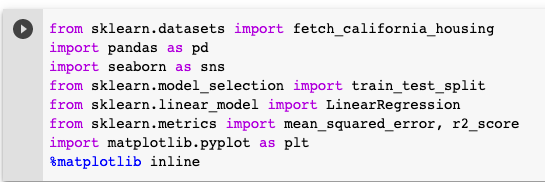
\includegraphics [scale=0.45]{figures/import_statements.png}}
	\caption{Import statements}
	\label{fig:placeholder}
\end{figure}
\section{Practical Example}
In this paper, the California housing datasets from \cite{KELLEYPACE1997291} included in the Scikit-Learn sklearn datasets library is used to train and predict the average prices of housing in California using linear regression. 
\subsection{Inspecting Dataset}
The dataset has 20,640 instance number, 8 numeric predictive attributes and 1 target attribute, i.e. the expected output of the prediction, which is the median house value for California districts. A block group is the smallest geographical unit for which the U.S. Census Bureau publishes sample data (a block group typically has a population of 600 to 3,000 people); the datasets were obtained in a 1990 census \cite{KELLEYPACE1997291}.
The predictive attributes have the following information: 
	\begin{itemize}
		\item MedInc: represents the median income in a block.
		\item HouseAge: represents the median house age in block.
    		\item AveRooms: represents the average number of rooms.
    		\item AveBedrms: represents the average number of bedrooms.
    		\item Population: represents the population in the block.
    		\item AveOccup: represents the average house occupancy.
	    \item Latitude: represents the house block latitude.
    		\item Longitude: represents the house block longitude.
	\end{itemize}
A summary of these attributes and the corresponding target values as pandas data frame is represented in figure \ref{fig:overview_dataset_with_target}. The target attribute represents the median house value in a unit of 100,000.

\begin{figure}[htbp]
	\centerline{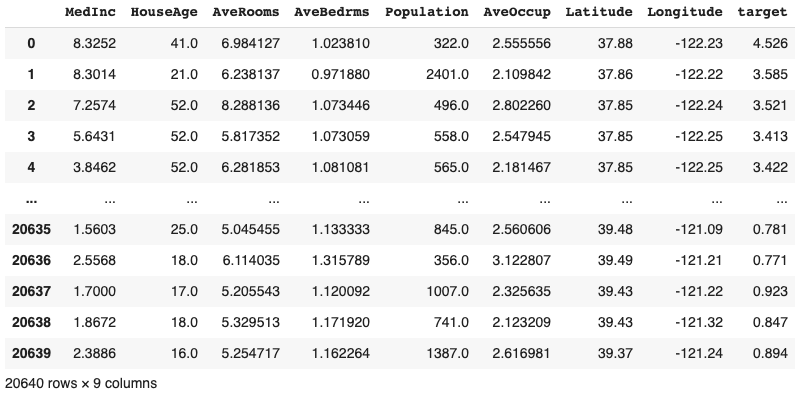
\includegraphics [scale=0.32]{figures/overview_dataset_with_target.png}}
	\caption{Dataset overview including the target column}
	\label{fig:overview_dataset_with_target}
\end{figure}

The correlation between the attributes is shown in figure \ref{fig:heatmap_correlation} and \ref{fig:Pearson_corr}. Figure \ref{fig:heatmap_correlation} shows the Pearson correlation between the attributes as a heatmap and figure \ref{fig:Pearson_corr} as a numerical table. The darker the blue colour and the closer the value is to 1, the higher the correlation of the attribute to each other. It can be seen from figure \ref{fig:heatmap_correlation} that the median income in a block has the highest correlation to the target value followed by house age and average rooms. The other values show little or no useful correlations to the target value because of their negative values.

\begin{figure}[htbp]
	\centerline{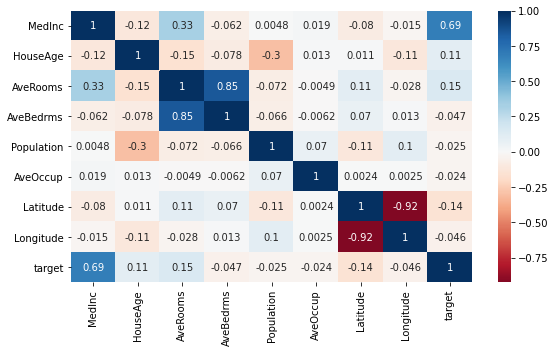
\includegraphics [scale=0.5]{figures/heatmap_correlation.png}}
	\caption{Pearson correlation heatmap of the dataset attributes}
	\label{fig:heatmap_correlation}
\end{figure}

\begin{figure}[htbp]
	\centerline{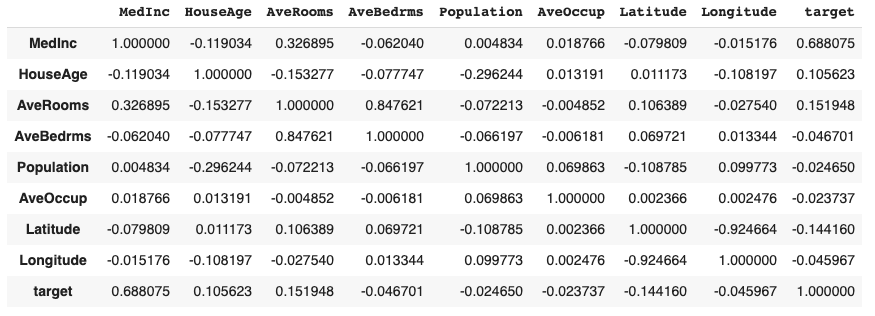
\includegraphics [width=90mm,scale=0.5,height=5cm]{figures/pearson_correlation_of_the_dataset.png}}
	\caption{Table of the Pearson correlation of dataset attributes}
	\label{fig:Pearson_corr}
\end{figure}



\subsection{Split Dataset and Train Model}
The dataset is split into training and testing data using the $train\_test\_split$ function provided by the $sklearn.model\_selection$ class. The dataset was split into 20\% - 4,218 - for testing purposes and 80\% -16, 512 - for training purposes. Splitting the dataset allows setting aside some dataset for testing purposes to evaluate the trained model's accuracy efficiently. If the dataset were not split, there is probability of the model predicting the target value through memorising and we want to avoid this. 

An instance of the linear regression model class was instantiated, and the training datasets were fed into the $fit$ function, which is an implementation of the linear regression formula. The value of the coefficients after training the model is [ 4.48674910e-01 9.72425752e-03 -1.23323343e-01 7.83144907e-01
 -2.02962058e-06 -3.52631849e-03 -4.19792487e-01 -4.33708065e-01]. The value of the intercept was found to be -37.023277706063894. Ideally, these are the values needed if a manual calculation of the target value $y$ is to be made. 

\subsection{Result and Discussion}
With the regression model successfully trained, the testing datasets can now be fed to the model to predict the target values. The coefficient of determination $R^2$ of training datasets for the model was found to be 0.6125511913966952.
When predictions were made using the testing dataset, there were some offsets in the predicted values to the target value as shown in figure \ref{fig:actual_vs_predicted} which shows a graph of the first 20 values. The Mean squared error of the predicted value to the target value was found to be 0.56 and the coefficient of determination to be 0.58. These values explain the reason why there were some offsets in the predictions.


\begin{figure}[htbp]
	\centerline{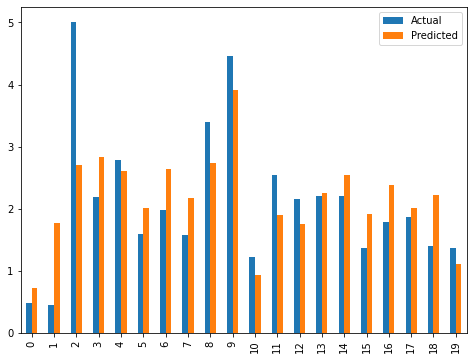
\includegraphics [scale=0.5]{figures/actual_vs_predicted.png}}
	\caption{Graph of first 20 actual values vs predicted values by the trained model}
	\label{fig:actual_vs_predicted}
\end{figure}

With the result of the predictions from the model, it can be said that the model has under fitted the training data because the features used did not have an accurate linear correlation. This can be seen in figure \ref{fig:Pearson_corr} which showed some negative values. We can also understand that many not-so-known factors influence house prices that were not included in the datasets or could not be found using linear regression.


\section{Conclusion}
The paper's primary aim is to understand linear regression in the context of machine learning and how to train a regression machine learning model to predict the average price of a house for a district block in California.

Different sections in the paper gave essential information on machine learning and linear regression to achieve this aim. A practical example was done using the different feature points that made up the California house price dataset utilising the Scikit learn python library, which implements the necessary mathematical formulas needed to make the statistical prediction job. The coefficient of determination of the training dataset was found to be $R^2$ = 0.6125511913966952. Predictions made using the testing dataset gave $R^2$ = 0.58 and mean squared error MSE = 0.56. These values showed that the model has around 57\% accuracy of correctly predicting the dependent variable.

In conclusion, as can be highlighted from the linear regression equation, it is a reasonably straightforward regression model to get started within machine learning. However, it is pretty poor at predicting datasets that do not have solid linear correlation as depicted in the trained model in this paper. As a suggestion, different regression algorithms should be tried out in training linearly related datasets to find the best fit for the desired prediction job.

\bibliographystyle{plain}
\bibliography{references}
\end{document}